\chapter{Dataset}
\section{Dataset: The Rosenwald Guides}
\subsection{Historical Context and Significance}
The \emph{Guides Rosenwald} are medical directories listing physicians and pharmacists in France and its colonies. Published annually between 1887 and 1949, the collection comprises 47 volumes. Originally conceived as a strategic reference work, the Guides aimed to provide a comprehensive overview of the medical profession across French territories to assist doctors and pharmacists in choosing their place of practice. Their stated mission was to regulate the spatial distribution of medical professionals so as to avoid overcrowding and ensure balanced access to care. As the preface to the 1887 edition states:

\begin{quote} ``Éviter un encombrement également préjudiciable aux nouveaux venus et aux médecins et pharmaciens déjà fixés.’’

\emph{— Préface du Guide Rosenwald (1887)} \end{quote}

However, it is worth emphasizing the directory’s highly practical utility for the general public: enabling users to find a specific physician in a given location. This utilitarian function is clearly reflected in the organization of the lists. Users could search for a doctor established in their neighborhood or even on their specific street (location-based lists), or locate the contact details of a known individual (alphabetical lists). Furthermore, specialized lists were provided for those seeking specific practitioners, such as surgeons, dentists, pharmacists, or doctors acting in thermal spas.


From a digital humanities perspective, this corpus constitutes a rich and still underexplored historical source for examining the geography of medical practice, the evolution of healthcare networks, and the social and institutional dynamics of French medicine in the late nineteenth and early twentieth centuries.

\clearpage
\subsection{Document Layout and Extraction Challenges}
Figure~\ref{fig:global} shows a double-page spread from the Rosenwald Guides. Our focus is on the doctor entries in red boxes; however, the pages also contain advertisements and other information. Figure~\ref{fig:close} illustrates the structure of typical entries. Several challenges arise: some fields are missing for certain individuals, line breaks cause entries to overlap in layouts. These noises present difficulties to our task of extracting structured information.

\begin{figure}[H]
\centering
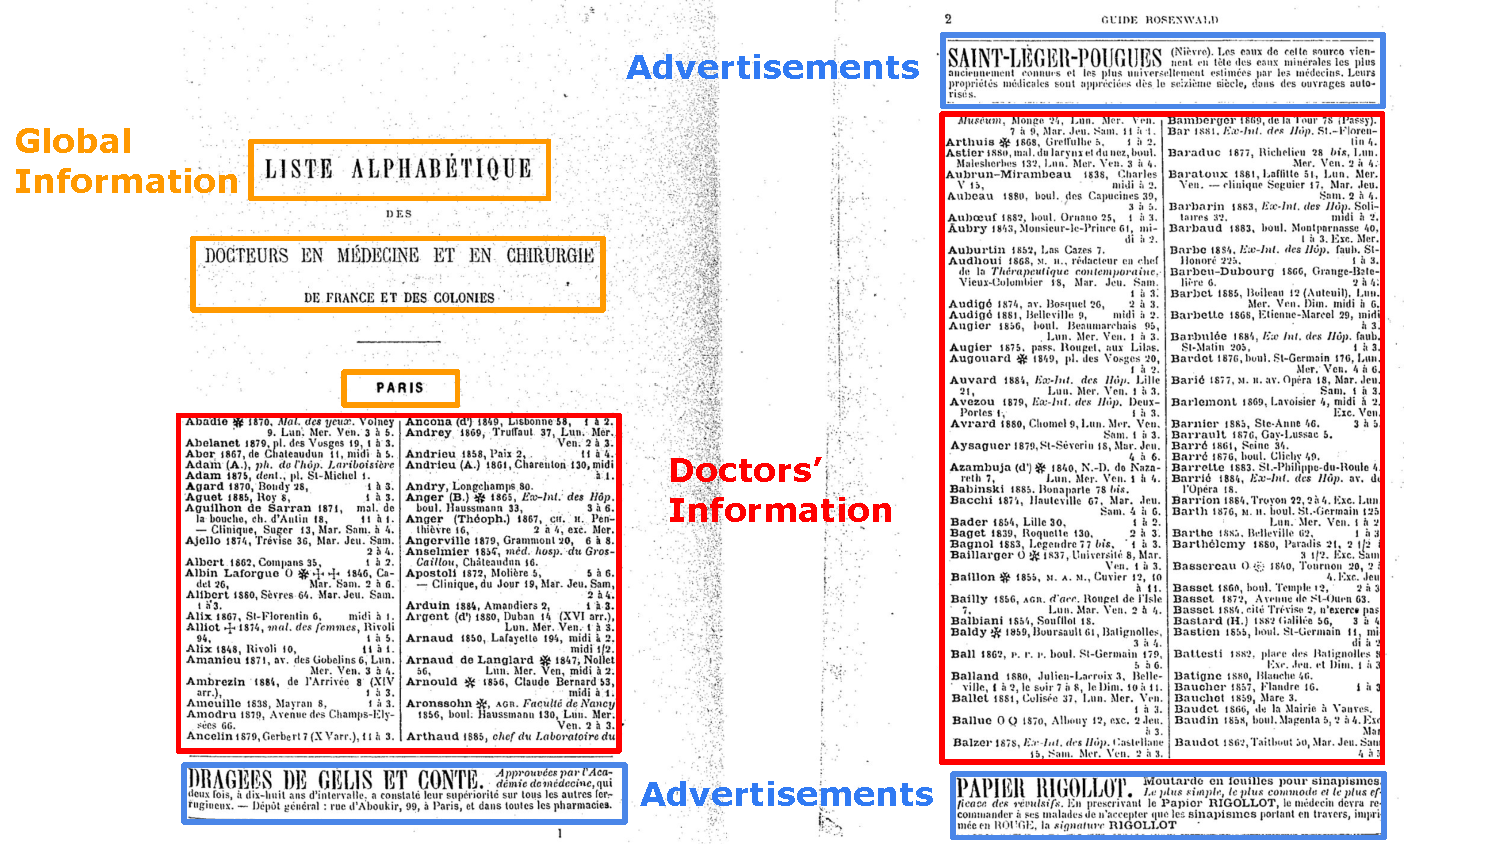
\includegraphics[width=\textwidth]{Images/global-page.pdf}
\caption{Page view of the Rosenwald Guide (1887, page 22–23)}
\label{fig:global}
\end{figure}

\begin{figure}[H]
\centering
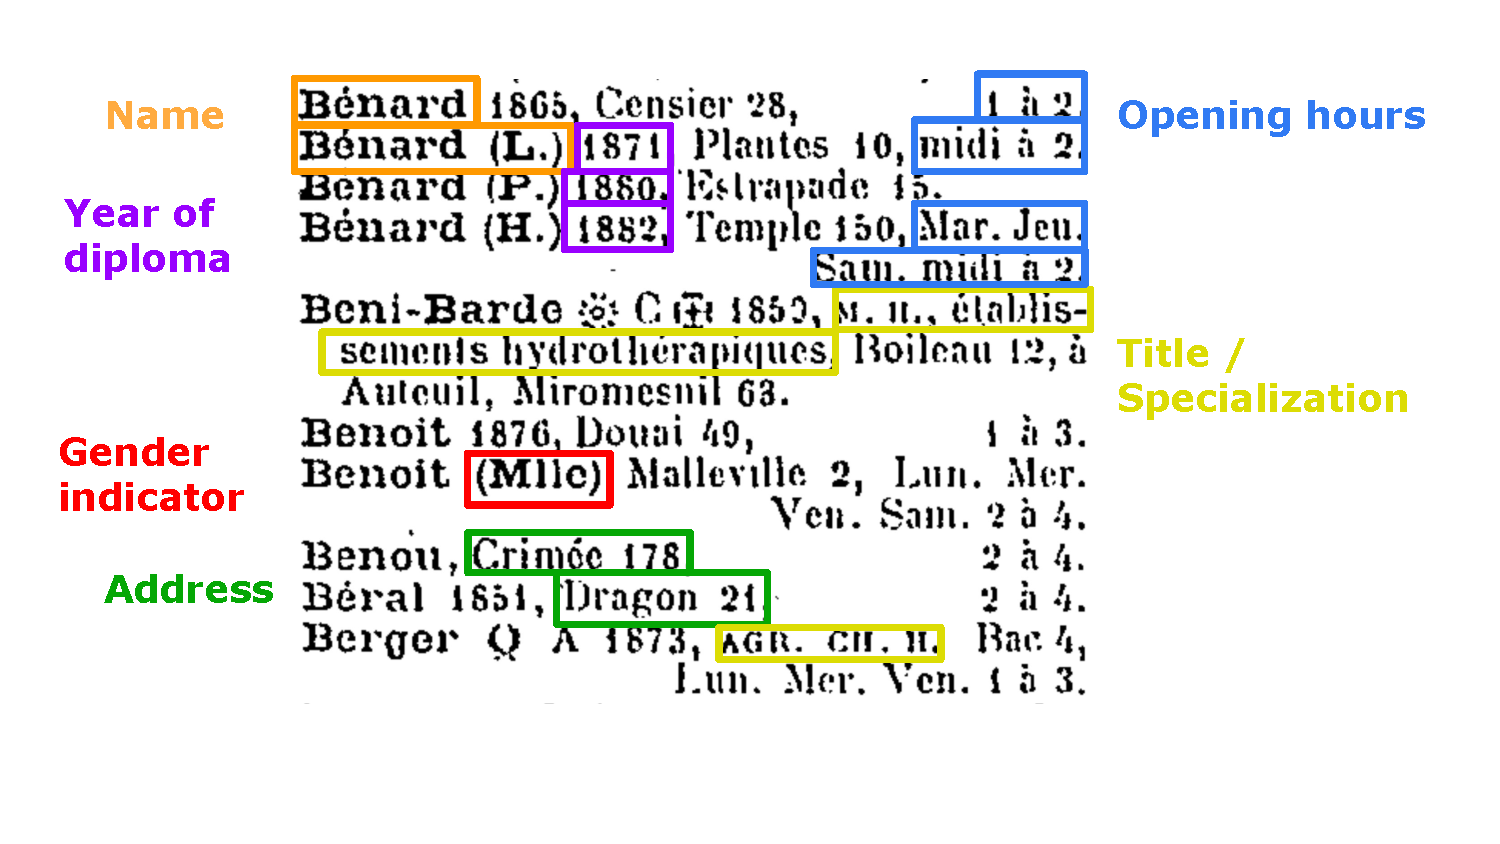
\includegraphics[width=0.9\textwidth]{Images/close-look.pdf}
\caption{Close-up of annotated entries in the Rosenwald Guide (1887, page 24)}
\label{fig:close}
\end{figure}


\subsection{Corpus Construction and Statistics}
\label{sec:corpus}
In this paper, we focus on extracting doctor entries, with particular attention to female doctors, for example, their name, year of diploma, specialization. Table~\ref{tab:medecins_b} shows an example extraction of Figure~\ref{fig:close}.

\begin{table}[htbp]
\centering
\small
\begin{tabular}{llp{3.2cm}p{2.3cm}p{3.5cm}l}
\toprule
\textbf{Nom} & \textbf{Année} & \textbf{Notes} & \textbf{Adresse} & \textbf{Horaires} & \textbf{Sexe} \\
\midrule
Bénard        & 1865 &  & Censier~28 & 1 à 2 &  \\
Bénard (L.)   & 1871 &  & Plantes~10 & midi à 2 &  \\
Bénard (P.)   & 1880 &  & Estrapade~15 &  &  \\
Bénard (H.)   & 1882 &  & Temple~150 & Mar.~Jeu.~Sam.~midi à 2 &  \\
Beni-Barde    & 1853 & M.~H., établissements hydrothérapiques & Boileau~12 (Auteuil), Miromesnil~63 &  &  \\
Benoit        & 1876 &  & Douai~49 & 1 à 3 &  \\
Benoit (Mlle) &  &  & Malleville~2 & Lun.~Mer.~Ven.~Sam.~2 à 4 & Mlle \\
Benou         &  &  & Crimée~178 & 2 à 4 &  \\
Béral         & 1851 &  & Dragon~21 & 2 à 4 &  \\
Berger        & 1873 & AGR.~CH.~H. & Bac~4 & Lun.~Mer.~Ven.~1 à 3 &  \\
\bottomrule
\end{tabular}
\caption{Doctor Entries of Figure~\ref{fig:close}}
\label{tab:medecins_b}
\end{table}


To narrow the scope of our analysis, we process only the sections titled \emph{Docteurs en médecine et en chirurgie} and \emph{Officiers de santé} for Paris and for the départements and colonies,  published between 1887 and 1906 (20 volumes). We manually identified the relevant page ranges for each volume and extracted the corresponding pages as images.

Table~\ref{tab:pages} presents the number of pages extracted for each edition, yielding a dataset of 4,116 pages in total. We can see that except for 1903 and 1904, each year has around 200 relevant pages.


\begin{table}[htbp]
\centering
\caption{Number of pages per edition of the Rosenwald Guides (1887–1906)}
\label{tab:pages}
\begin{tabular}{c c c c c c c c c c c}
\toprule
Year  & 1887 & 1888 & 1889 & 1890 & 1891 & 1892 & 1893 & 1894 & 1895 & 1896 \\
Pages & 202  & 186  & 187  & 183  & 183  & 184  & 190  & 191  & 189  & 216 \\
\midrule
Year  & 1897 & 1898 & 1899 & 1900 & 1901 & 1902 & 1903 & 1904 & 1905 & 1906 \\
Pages & 208  & 192  & 198  & 197  & 201  & 206  & 304  & 301  & 222  & 226 \\ 
\bottomrule
\end{tabular}
\end{table}



% \section{Dataset: The Rosenwald Guides}

% The \emph{Guides Rosenwald} are medical directories listing physicians in France and its colonies. 
% Published annually between 1887 and 1940, the corpus comprises 47 volumes, each of approximately one thousand pages. 
% Originally conceived as a practical reference for doctors and pharmacists when choosing their place of practice, the Guides aimed to provide a comprehensive overview of the medical profession across the French territories.

% Their stated mission was not only to inform but also to regulate the spatial distribution of medical professionals in order to prevent overcrowding and unequal access to care. As the preface to the first edition emphasizes:

% \begin{quote}
% ``Éviter un encombrement également préjudiciable aux nouveaux venus et aux médecins et pharmaciens déjà fixés.’’\\
% \emph{— Préface du Guide Rosenwald (1887)}
% \end{quote}


% From a digital humanities perspective, this corpus constitutes a rich and underexplored historical source for studying the geography of the medical profession, the evolution of healthcare networks, and the social and institutional dynamics of French medicine during the late nineteenth and early twentieth centuries.


% Figure \ref{fig:global} displays two pages of the Rosenwald Guides. We only want the doctors' information in the red boxes, but we also have advertisements and global information in the pages. Figure \ref{fig:close} explains the fields of doctor entries in Rosenwald Guides. It is illustrated that some fields are missing for some doctors, and the layout of the entries mix with each other when one row cannot hold all the characters. The noise in our data presents a challenge for structured information extraction.

% \begin{figure}[h]
%     \centering
%     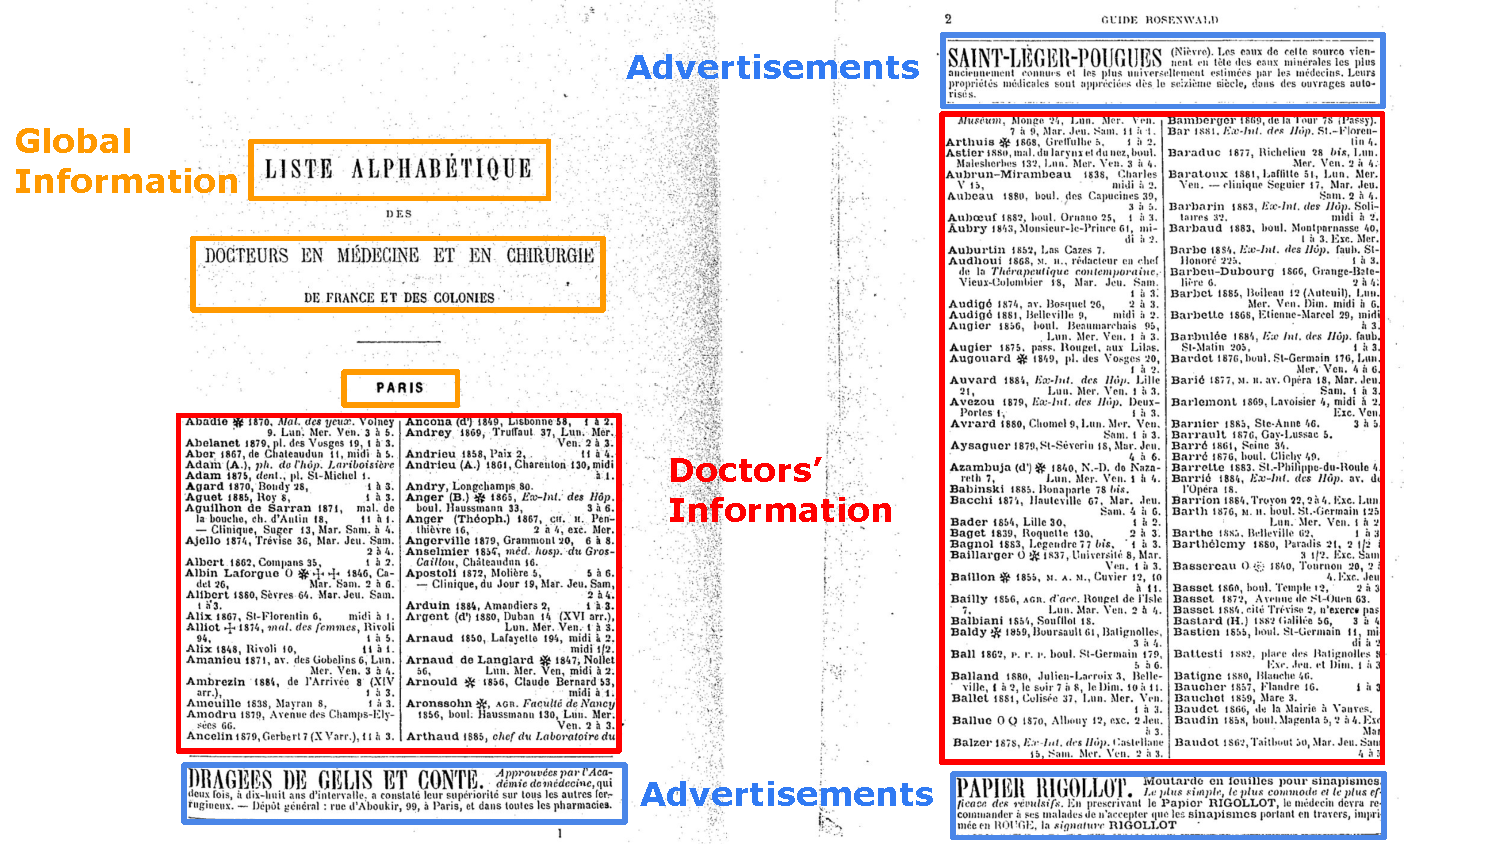
\includegraphics[width=\textwidth]{Images/global-page.pdf}
%     \caption{Page view of the Rosenwald Guide (1887, page 22 - 23)}
%     \label{fig:global}
% \end{figure}

% \begin{figure}[h]
%     \centering
%     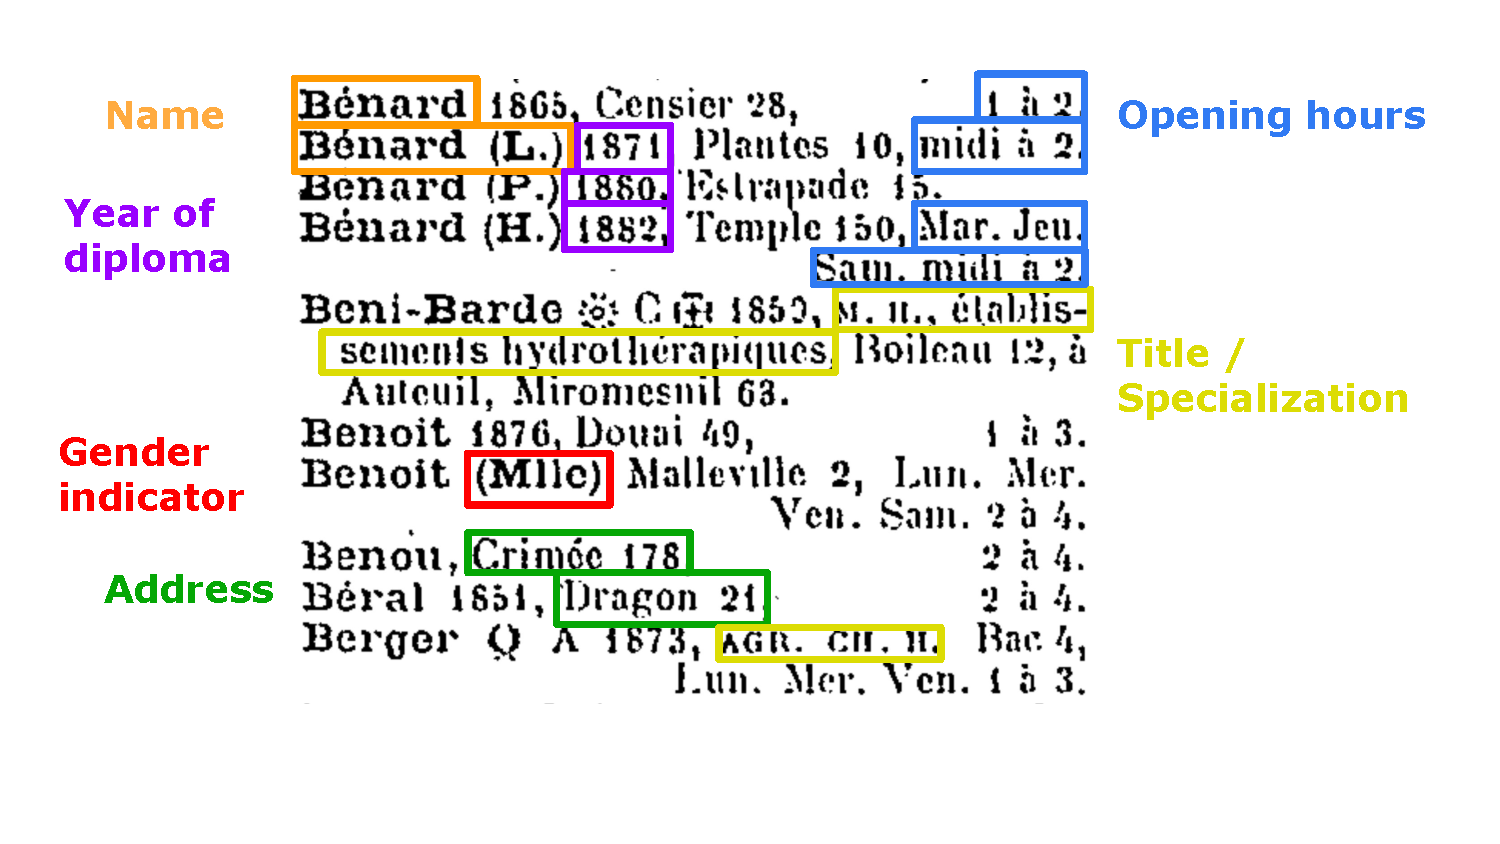
\includegraphics[width=\textwidth]{Images/close-look.pdf}
%     \caption{Explanation of some entries in the Rosenwald Guide (1887, page 24)}
%     \label{fig:close}
% \end{figure}


% In our paper, we focus on extracting the doctors, with a particular focus on female doctors, from 20 books (1887-1906). To make our research focused, we only process the list of DOCTEURS EN MÉDECINE ET EN CHIRURGIE and OFFICIERS DE SANTÉ of Paris and DEPARTEMENT ET COLONIES. We manually identified corresponding pages and extracted them into images.

% Table \ref{tab:pages} shows the count of extracted pages, 4116 pages in total

